\selectlanguage{magyar}
\enfalse
\hutrue
\pagenumbering{gobble}
%--------------------------------------------------------------------------------------
% Nyilatkozat
%--------------------------------------------------------------------------------------
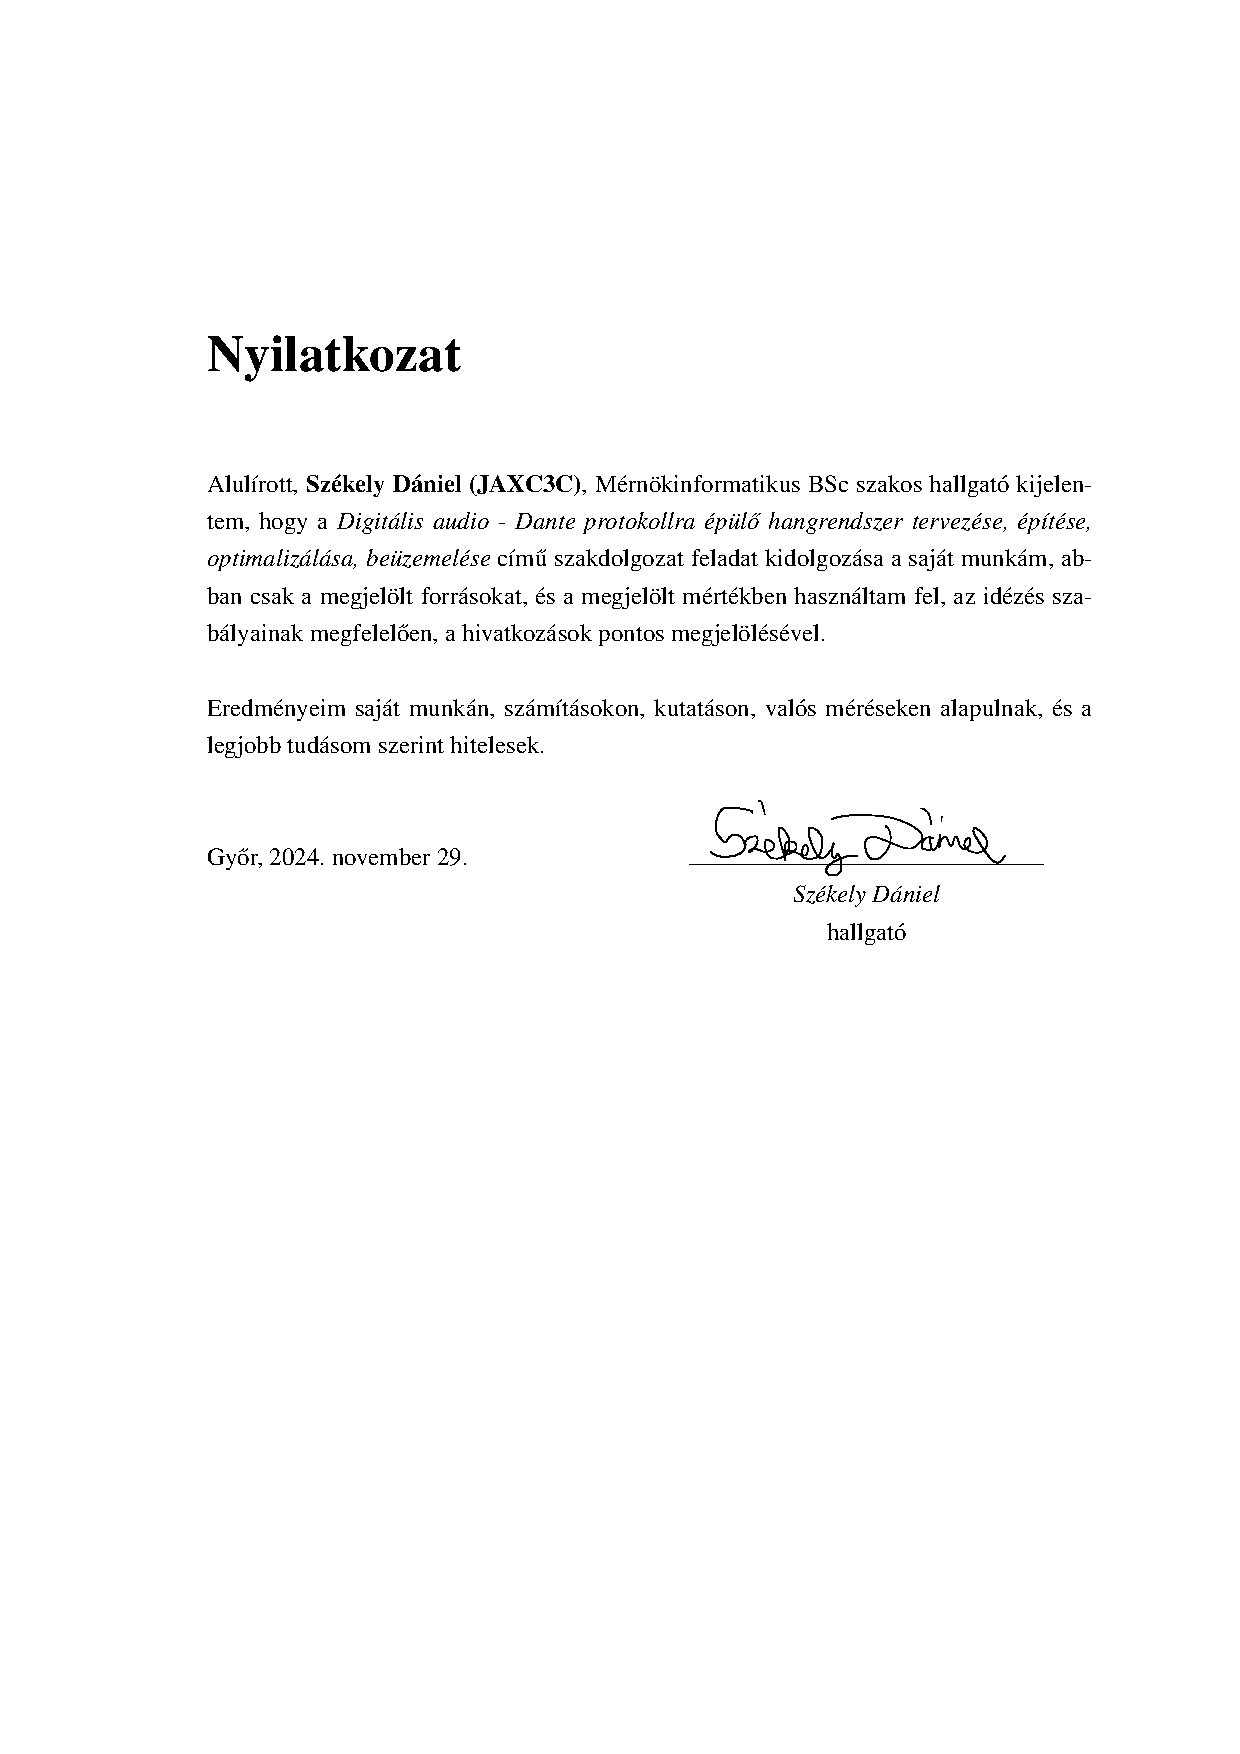
\includepdf{figures/nyilatkozat.pdf}
\begin{comment}
\noindent
Alulírott, \textbf{\szerzoVezeteknev{} \szerzoKeresztnev{} (\szerzoNeptun)}, \szak{} szakos hallgató kijelentem, hogy a \textit{\cim} című \MakeLowercase{\doktipus{}} feladat kidolgozása a saját munkám, abban csak a megjelölt forrásokat, és a megjelölt mértékben használtam fel, az idézés szabályainak megfelelően, a hivatkozások pontos megjelölésével.

\setlength\parskip{\baselineskip}

\noindent
Eredményeim saját munkán, számításokon, kutatáson, valós méréseken alapulnak, és a legjobb tudásom szerint hitelesek.

\vspace*{24pt}
\begin{multicols}{2}
	\noindent
	Győr, \emitdate{b}{\today}

	\columnbreak
	\noindent
	\makebox[7cm][c]{\rule{6cm}{.4pt}}\\
	\makebox[7cm][c]{\emph{\szerzoVezeteknev{} \szerzoKeresztnev}}\\
	\makebox[7cm]{hallgató}
\end{multicols}
\end{comment}

\thispagestyle{empty}

\vfill
\clearpage
\thispagestyle{empty} % an empty page

\selectthesislanguage
